\newpage
\textbf{Tables}
\begin{table}[ht]
    \caption{MRI acquisition parameters. The GE dataset Axial and Sagittal series were acquired in two fields of view (FOV): large field of view (LFOV) and small field of view (SFOV). The Siemens dataset, was only acquired in the SFOV modality.}
    \begin{tabular}{lcccccc}
         \hline
          \textbf{Magnet} & \textbf{Plane} & \textbf{FOV} & \textbf{TE Min - Max} & \textbf{TR Min - Max} & \textbf{Matrix} & \textbf{Voxel size (mm)} \\
          GE & Axial & LFOV (n=100) & $81.31 - 105.50$ & $4806 - 10998$ & $256 \times 256 \times 72$ & $1.25 \times 1.25 \times 2.5$ \\
          GE & Axial & SFOV (n=120) & $80.88 - 93.48$ & $3700 -7078$ &
                \shortstack{ $256 \times 256 \times 27$ to\\ $512 \times 512 \times 37$} & 
                \shortstack{ $0.3906 \times 0.3906 \times 3$ to\\ $0.7813 \times 0.7813 \times 3$} \\
          GE & Coronal & SFOV (n=220) & $80.49 - 134.17$ & $1968 - 8006$ &  
                \shortstack{$320 \times 320 \times 32$ to \\  $512 \times 512 \times 30$} & 
                \shortstack{$0.3906 \times 0.3906 \times 3$ to \\ $0.6875 \times 0.6875 \times 3$}\\
          GE & Sagittal & LFOV (n=25) & $88.32 - 94.70$ & $9000$ & 
                \shortstack{$512 \times 512 \times 25$ to \\  $512 \times 512 \times 40$} & 
                $0.429688 \times 0.429688 \times 3$\\
          GE & Sagittal & SFOV (n=195) & $80.49 - 134.51$ & $2124 - 7917$&  
                \shortstack{ $256 \times 256 \times 25$ to \\ $512 \times 512 \times 33$} &
                \shortstack{$0.3906 \times 0.3906 \times 3$ to \\ $0.7813 \times 0.7813 \times 3$}\\
          Siemens & Axial & SFOV (n=330)  & $101 - 108$ & $4030 - 8624$&  
                \shortstack{$256  \times 256 \times 17$ to \\ $640 \times 640 \times 23$} & 
                \shortstack{$0.3906 \times 0.3906 \times 3$ to\\ $0.7813 \times 0.7813 \times 3$} \\
          Siemens & Coronal & SFOV (n=330) & $97 - 110$ & $3080 - 6620$&  
                \shortstack{$256  \times 256 \times 19$ to \\ $320 \times 320 \times 23$} & 
                \shortstack{$0.5625 \times 0.5625 \times 3$ to\\ $0.8001 \times 0.8001 \times 4$} \\
          Siemens & Sagittal & SFOV (n=330) & $101 - 110$ & $3810 - 6830$&  
                \shortstack{$320  \times 320 \times 17$ to \\ $448 \times 390 \times 13$} &
                \shortstack{$0.5625 \times 0.5625 \times 3$ to\\ $0.571 \times 0.571 \times 4$} \\
         \hline
    \end{tabular}
    Abbreviations: TE=Echo Time, TR=Repetition Time, FOV=Field of View, SFOV=Small Field of View, LFOV=Large Field of View
    \label{tab:dataset}
zr\end{table} 

\newpage
\begin{table}[ht]
    \caption{Dice Similarity Coefficients (DSC) (mean $\pm$ SD) for prostate, segmented with each of the three trained models (GE, Siemens, and Combined). The results are presented for data from GE and Siemens MRI vendors and the DSCs are calculated on the interpolated (0.5 x 0.5 x 0.5 mm) and original MRI resolution.}
    \begin{tabular}{lcc}
         \hline
          \textbf{Prostate Models} & \textbf{GE (Interpolated/Original Resolution)} & \textbf{Siemens (Interpolated/Original Resolution)}\\
         \hline
         GE & $0.855\pm0.064$/$\mathbf{0.860\pm0.054}$ & $0.804\pm0.099$/$0.802\pm0.106$ \\
         \hline
         Siemens & $0.262\pm0.118$/$0.288\pm0.139$ & $0.892\pm0.038$/$0.889\pm0.035$ \\
         \hline
         Combined & $0.830\pm0.112$/$0.827\pm0.109$ & $\mathbf{0.896\pm0.037}$/$0.892\pm0.036$\\
         \hline
    \end{tabular}
    \label{tab:res_prost}
\end{table} 

\newpage
\begin{table}[ht]
     \caption{Dice Similarity Coefficients (DSC) (mean $\pm$ SD) for PZ, segmented with each of the three trained models (GE, Siemens, and Combined). The results are presented for data from GE and Siemens MRI vendors and the DSCs are calculated on the interpolated (0.5 x 0.5 x 0.5 mm) and original MRI resolution.}
    \begin{tabular}{lcc}
         \hline
            \textbf{PZ Models} & \textbf{GE (Interpolated/Original Resolution)} & \textbf{Siemens (Interpolated/Original Resolution)}\\
         \hline
         GE  & $0.767\pm0.093$/$0.759\pm0.089$ & $0.537\pm0.204$/$0.539\pm0.204$ \\
         \hline
         Siemens  & $0.591\pm0.223$/$0.591\pm0.219$ & $0.808\pm0.085$/$0.808\pm0.087$ \\
         \hline
         Combined & $\mathbf{0.797\pm0.093}$/$0.788\pm0.093$ & $\mathbf{0.813\pm0.079}$/$0.811\pm0.79$\\
         \hline
    \end{tabular}
    \label{tab:res_pz}
\end{table}

\newpage
\textbf{Figure legends:}
\begin{figure}[ht]
    \centering
    %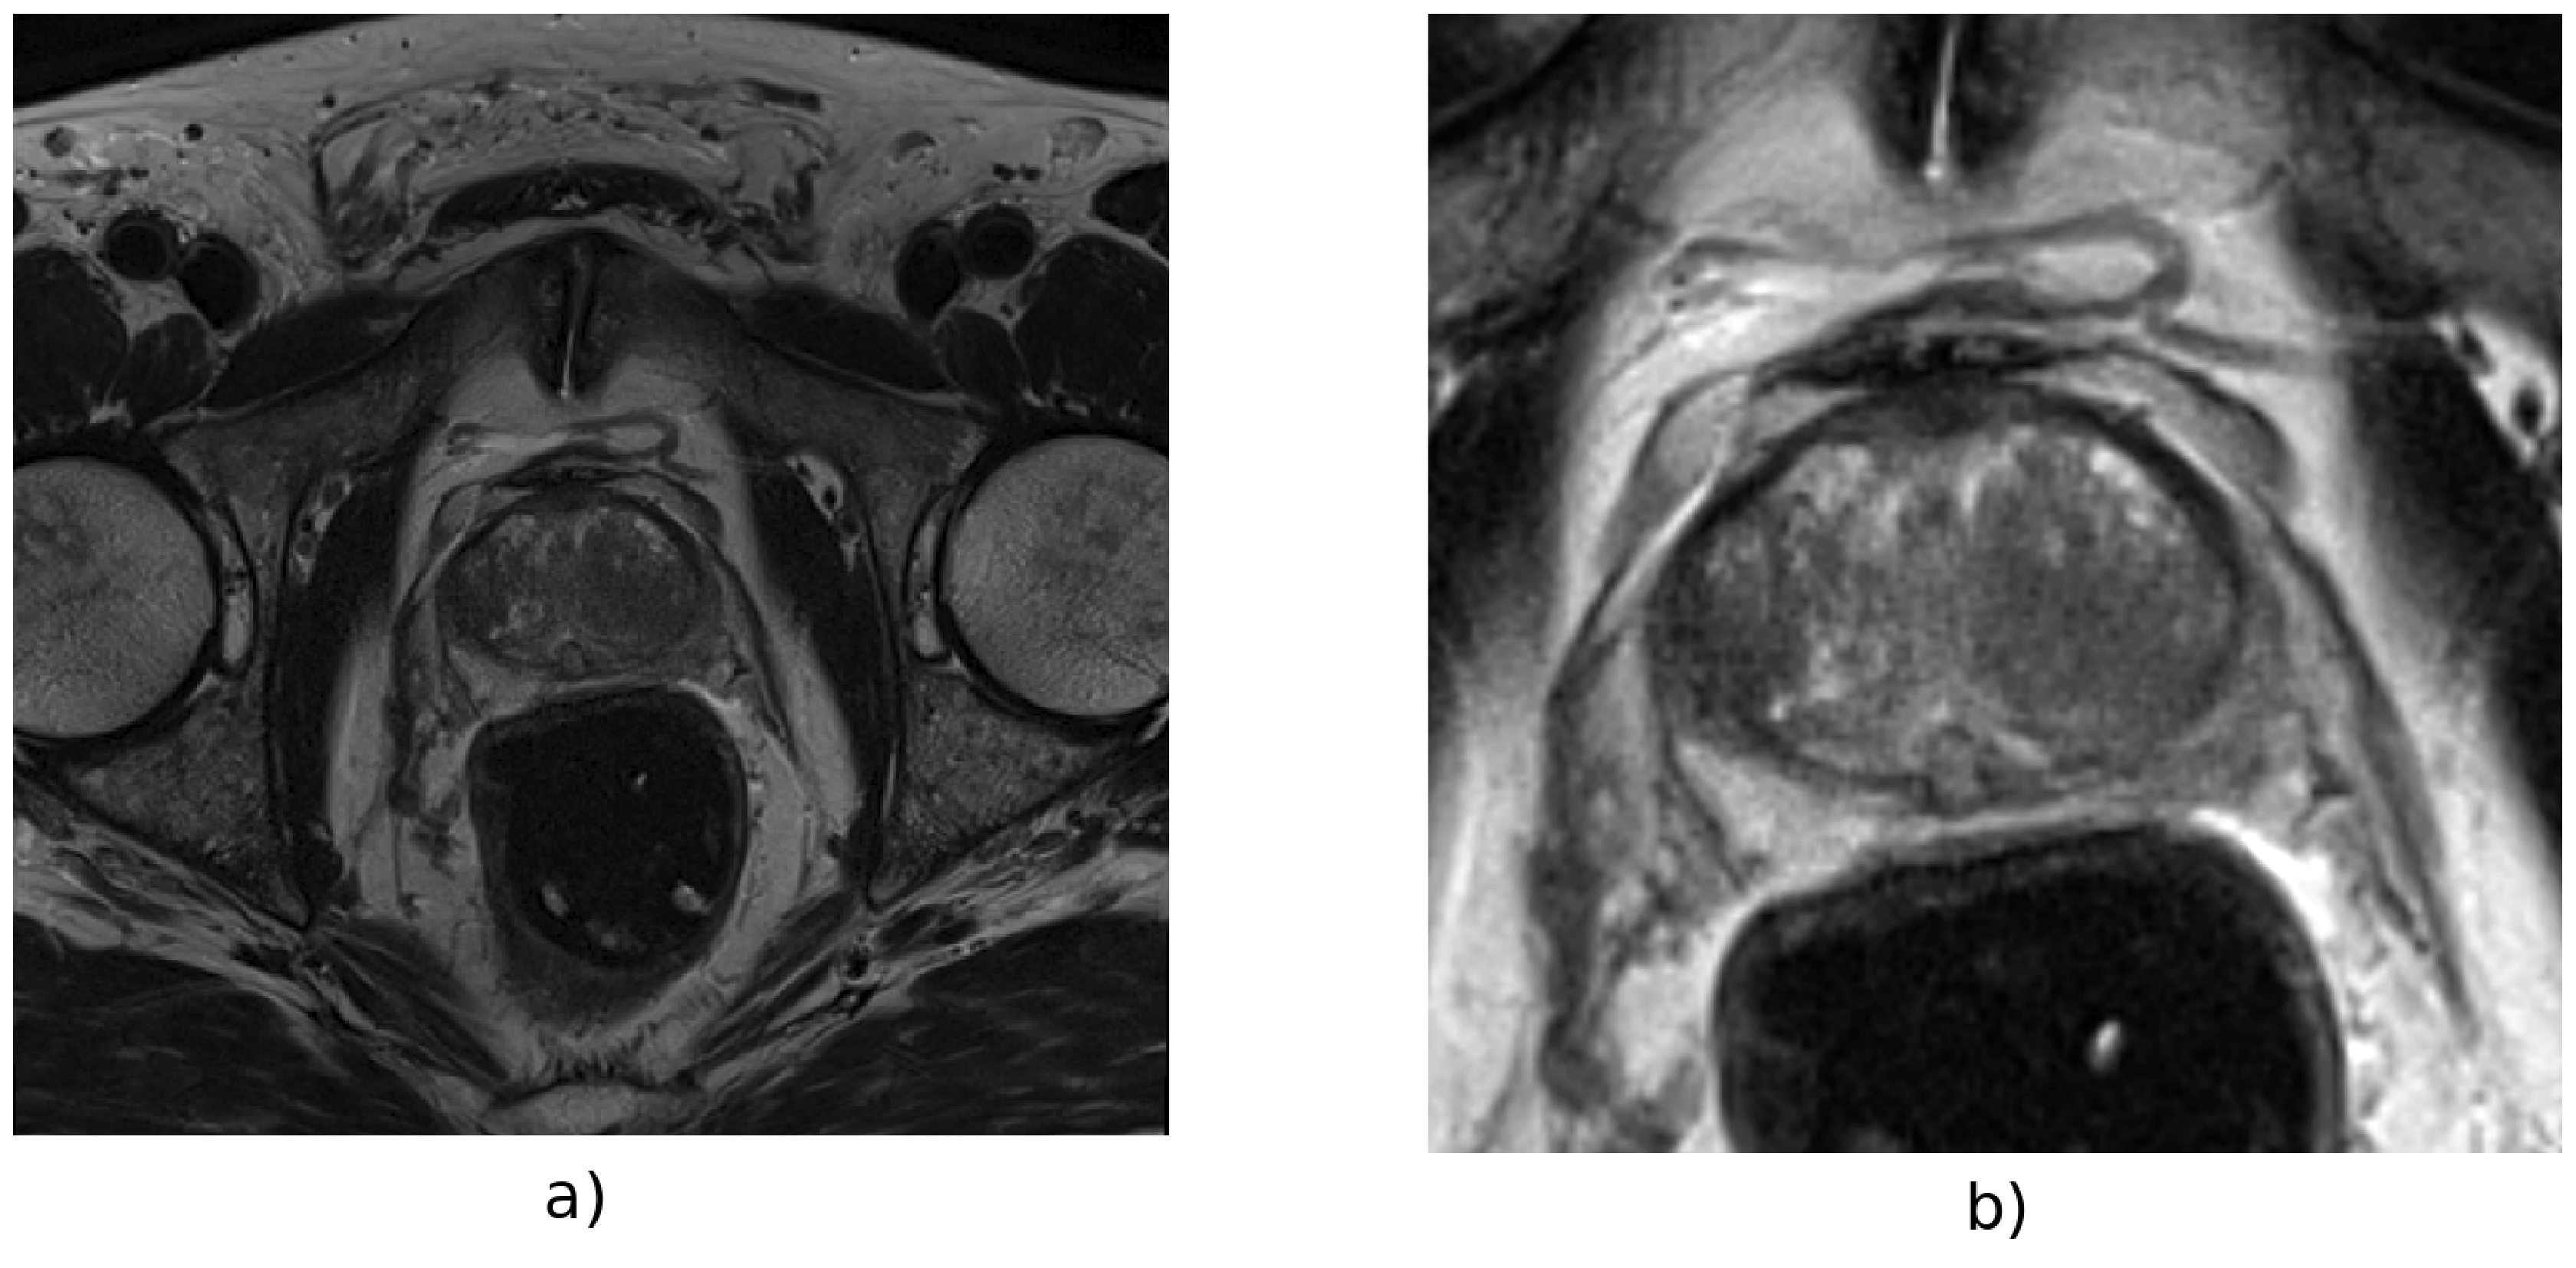
\includegraphics[totalheight=.25\textheight]{figures/Figure1.eps}
    \caption{Axial T2-weighted image \textbf{a)} before, and \textbf{b)} after preprocessing. Preprocessing steps include bias correction, intensity normalization, resampling, and cropping.} 
    \label{fig_1}
\end{figure}

\begin{figure}[ht]
    \centering
    %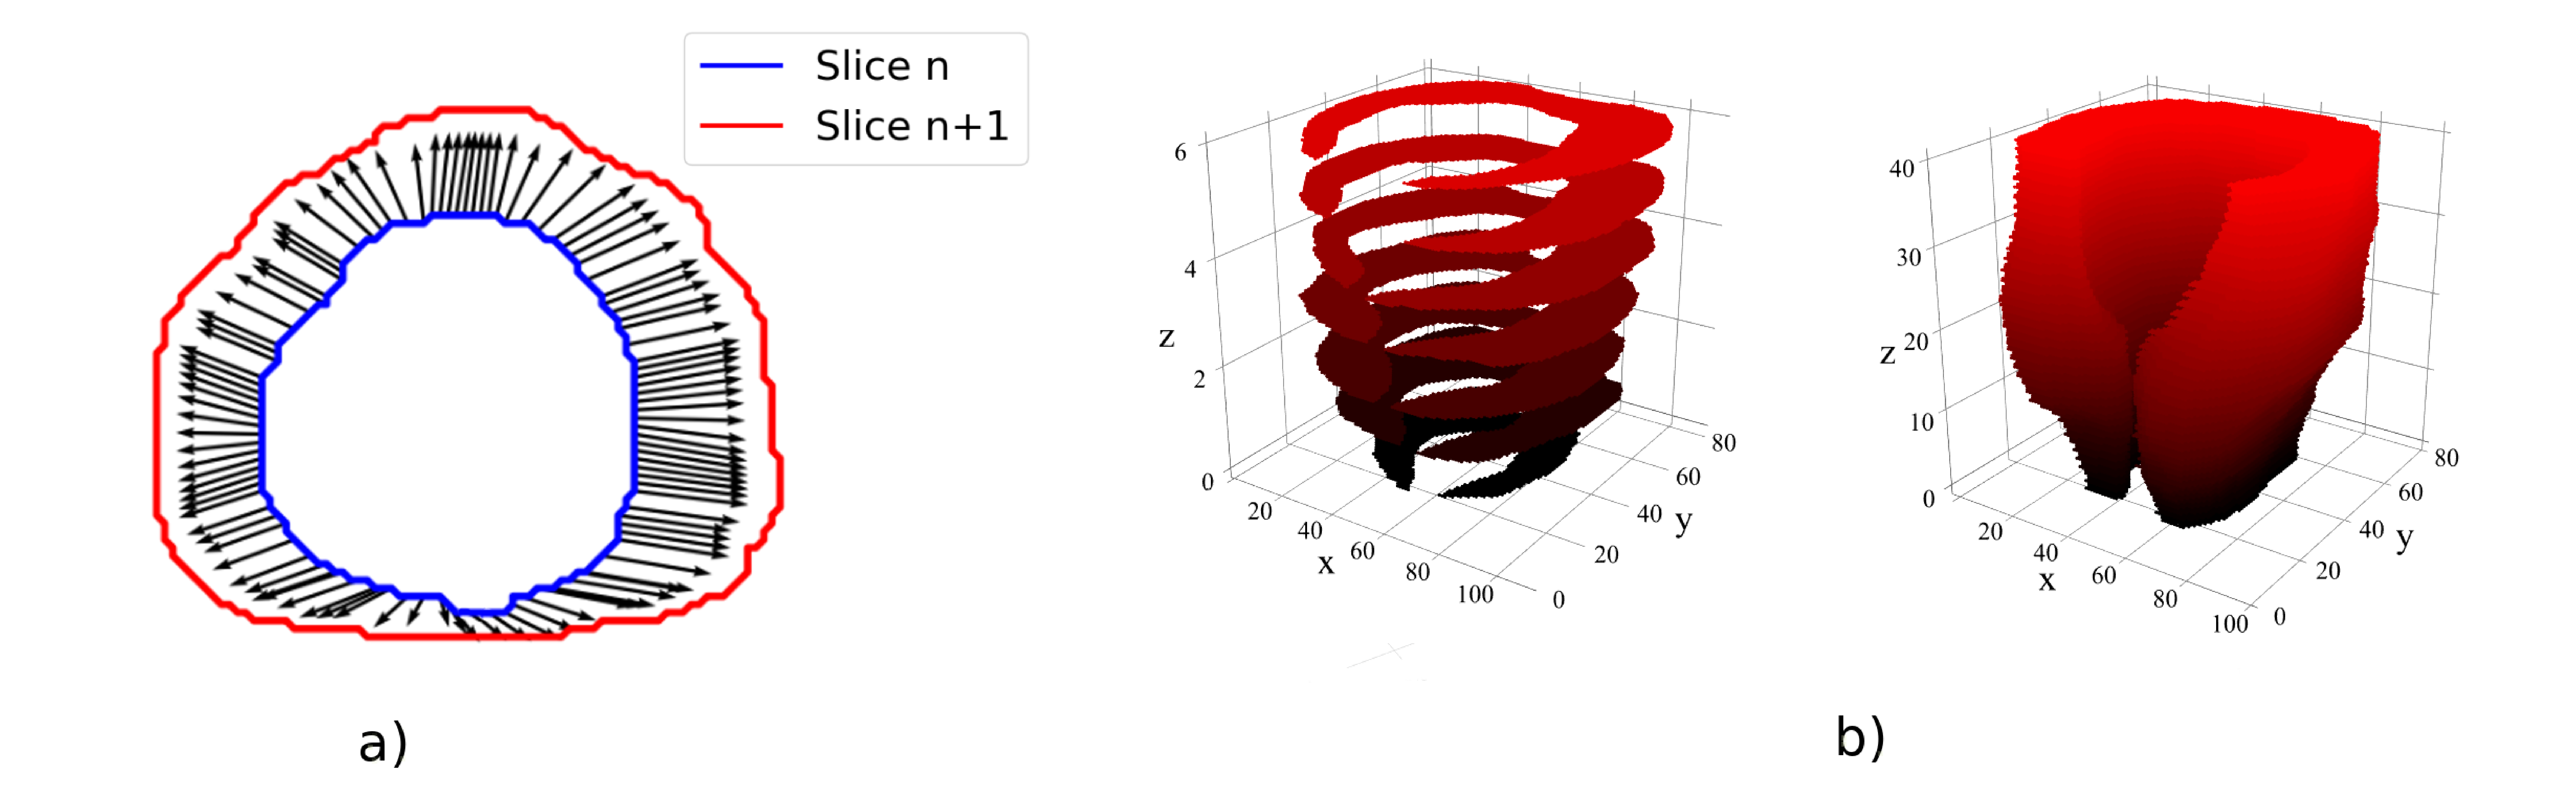
\includegraphics[totalheight=.21\textheight]{figures/Figure2.eps}
    \caption{Interpolation of prostate and PZ contours. \textbf{a)} an example of the optical flow obtained between two prostate contours from adjacent horizontal planes. In \textbf{b)} on the left, original PZ contours with 7 slices. On the right, interpolated contours with 40 slices.}
    \label{fig:fig_2}
\end{figure}

\begin{figure*}[ht]
    \centering
    %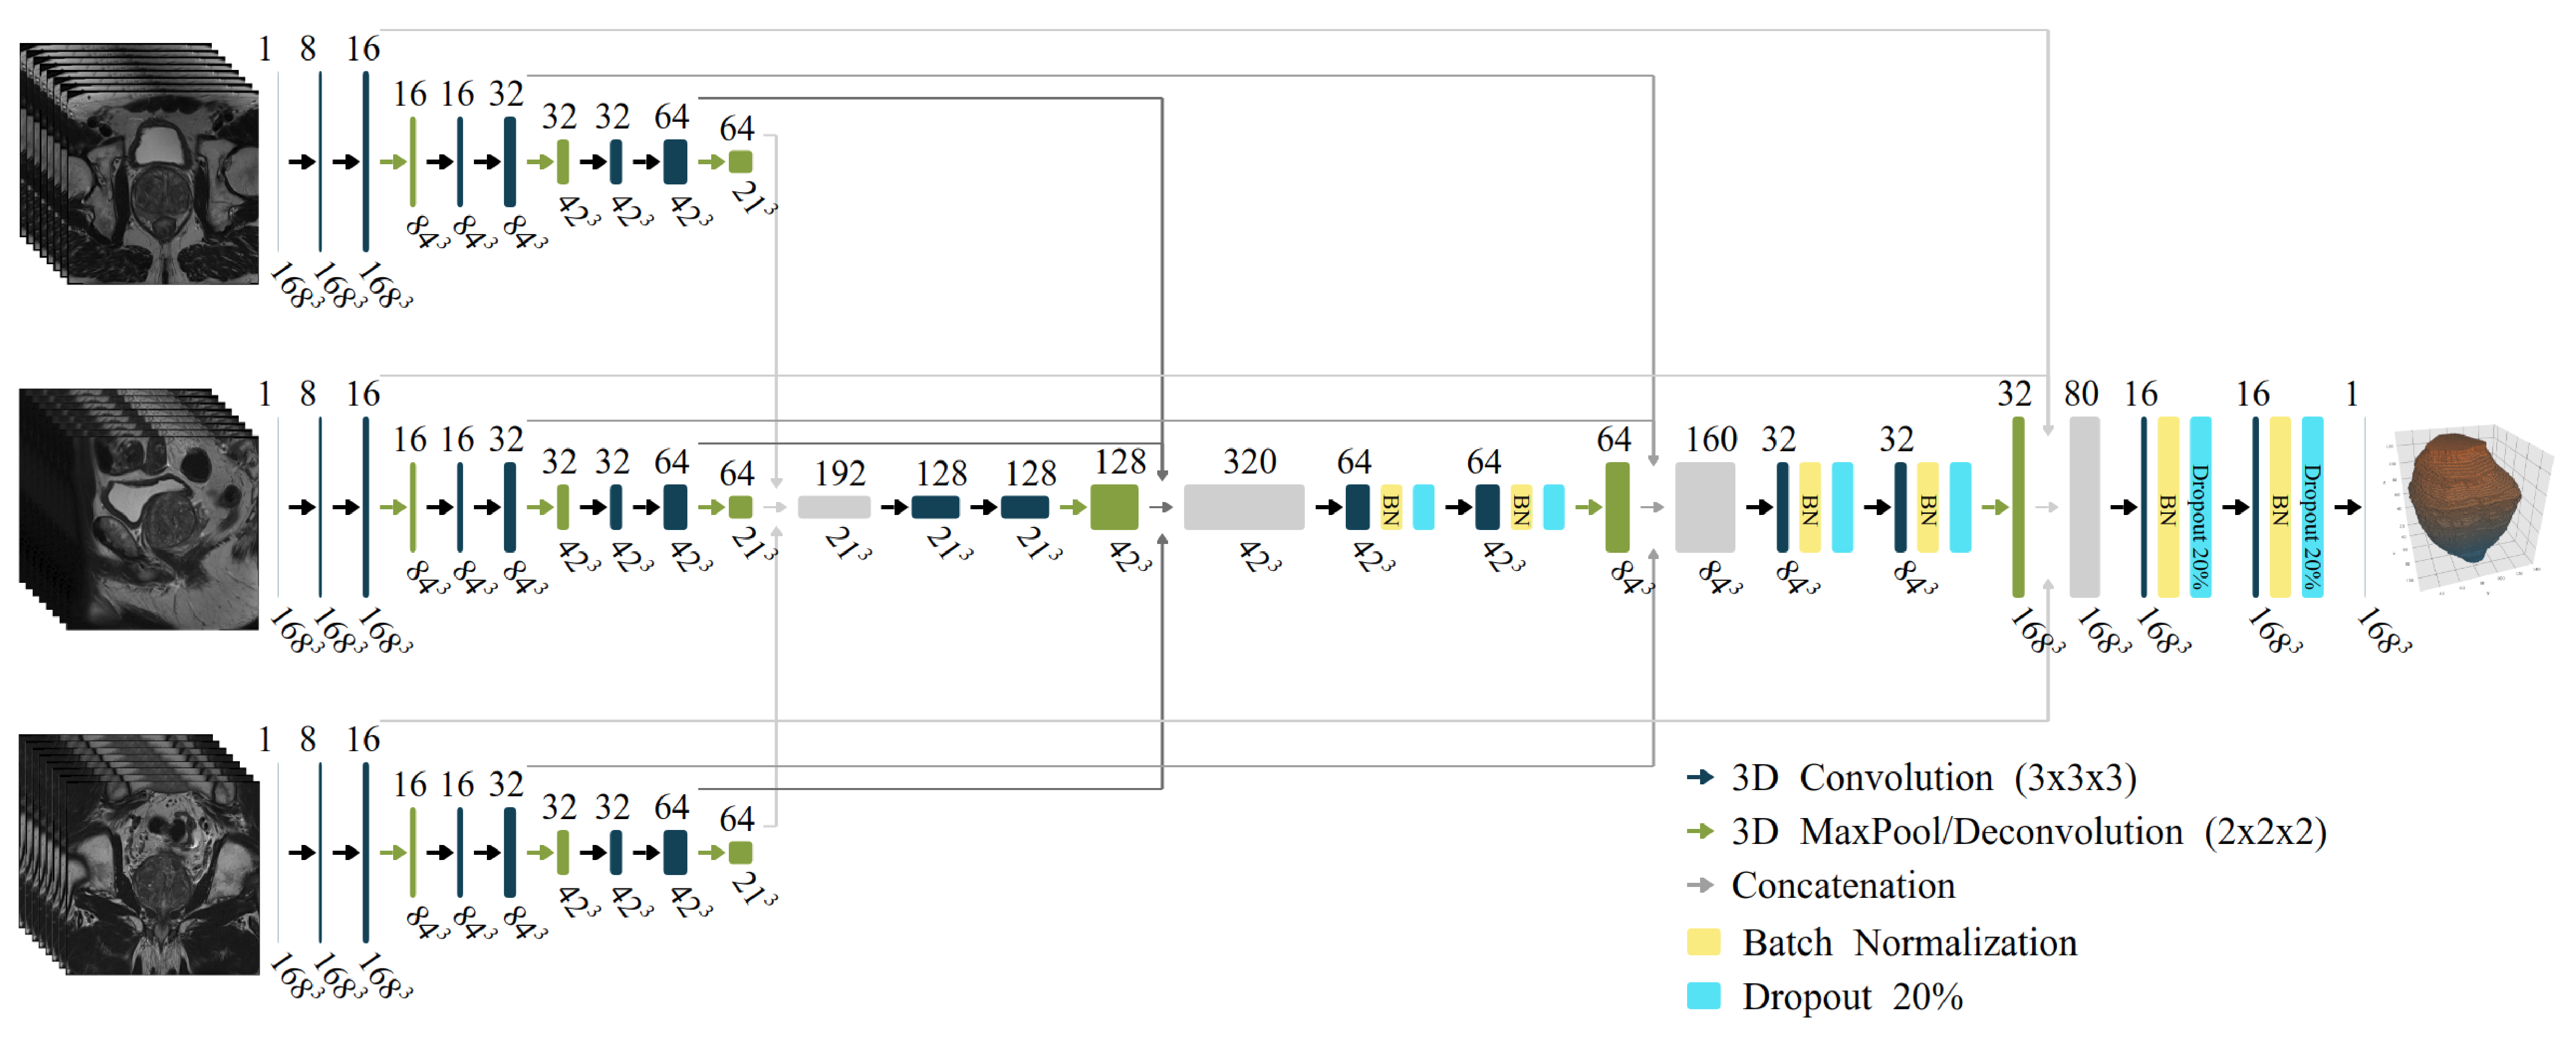
\includegraphics[totalheight=.282\textheight]{figures/Figure3.eps}
    \caption{Multistream 3D convolutional network architecture. The input of the network are three $168^3$ volumes from the MRI planes: axial, sagittal, and coronal. }
    \label{fig:fig_3}
\end{figure*}

\begin{figure}[ht]
    \centering
    %\includegraphics[totalheight=.45\textheight]{figures/Figure4.eps}
    \caption{Prostate segmentation for the cases with the lowest, closest to mean, and highest 3D DSC for the Siemens (up) and GE (down) datasets. These segmentation are obtained with the \emph{Combined} network model. Ground
    truth contours (GT) are in red and predicted  contours  (NN) are in yellow. }
    \label{fig:resseg}
\end{figure} 

\begin{figure}[ht]
    \centering
    %\includegraphics[totalheight=.45\textheight]{figures/Figure5.eps}
    \caption{Peripheral zone segmentation for the cases with the lowest, closest to mean, and highest 3D DSC for the Siemens (up) and GE (down) datasets. These segmentation are obtained with the \emph{Combined} network model. 
    Ground truth PZ contours (GT) are displayed in red, predicted  contours (NN) in cyan, and prostate contours in yellow.
    }
    \label{fig:ressegpz}
\end{figure} 

\begin{figure*}[ht]
    \centering
    %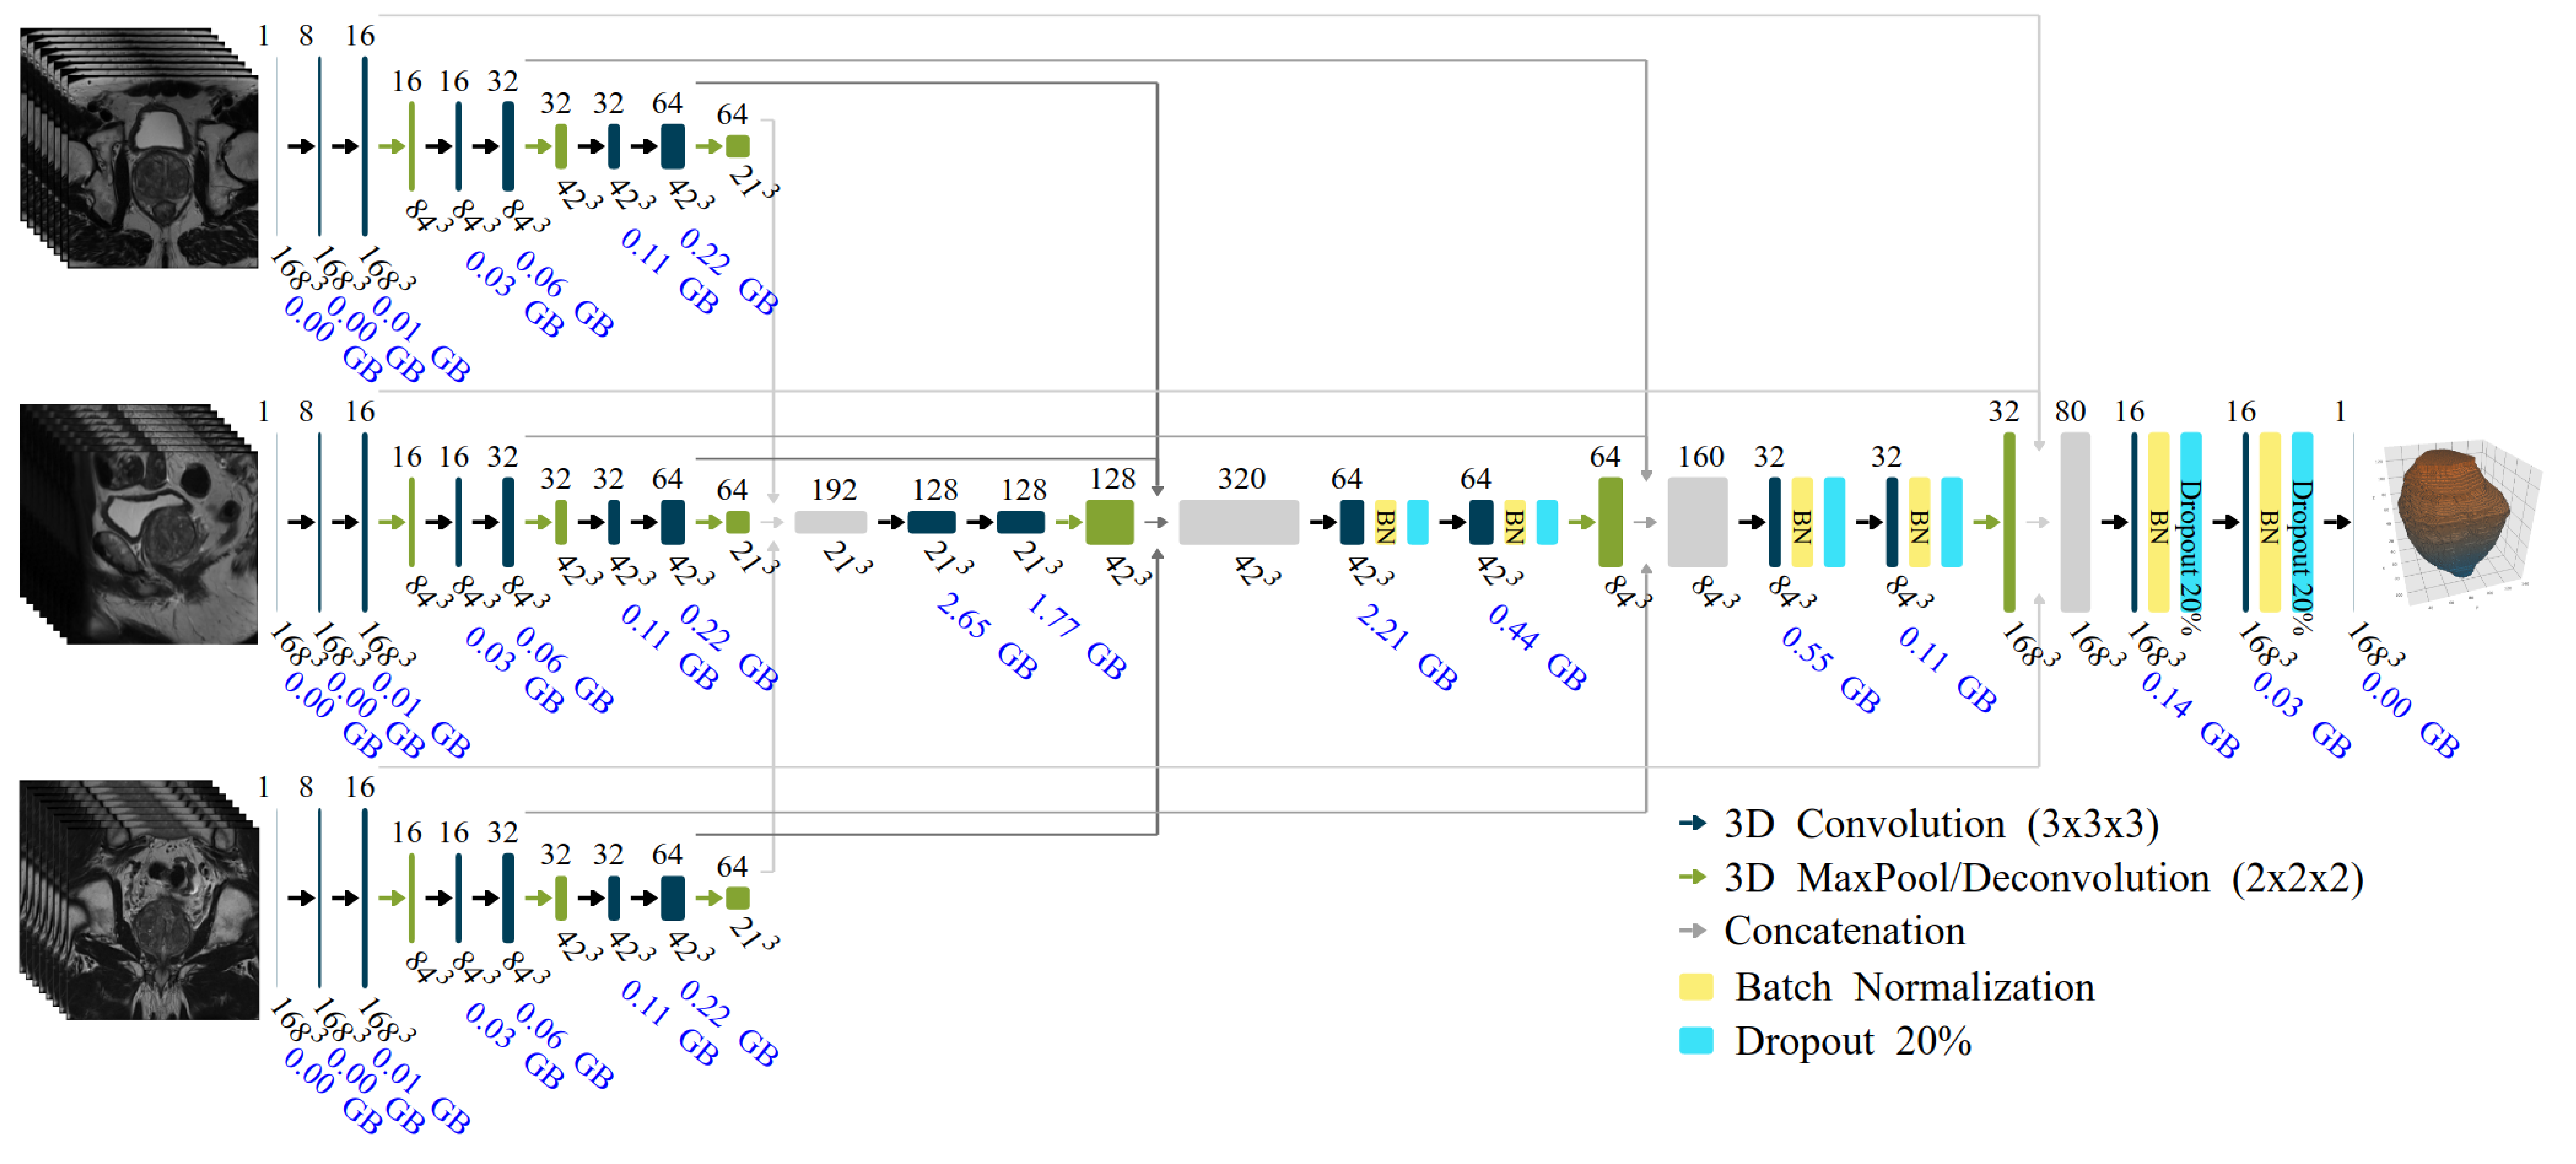
\includegraphics[totalheight=.32\textheight]{figures/Figure6.eps}
    \caption{Estimated amount of memory required to store the parameters of the proposed model at each convolutional layer. The memory size is displayed in gigabytes (GB). }
    \label{fig:nn_size}
\end{figure*}
